\chapter{Software operations}
\label{chap:soptware_operations}

\section{SetClock}
\label{operation:CloseCrisis}

An activator sets the date and time information in the system's State.

\begin{description}
	\item \textbf{Parameters:} DateAndTime
	\item \textbf{Precondition:} The system is initialized and the date and time
	value is greater than the one known by the system.
	\item \textbf{Post-condition:} The clock attribute of the State instance is
	updated to the given date and time.
	\item \textbf{Output messages:} "Date and time was updated
	successfuly".
	
	\item \textbf{Triggering:}
	
	\begin{enumerate}
		\item Choose a date in the entry "Date" or press the button "Now" to choose
		the current date.
		\item Choose hour, minute and second from the realated entries using
		scrollbars or filling in manually the entries.
		\item Press on the button "Change date and time".
	\end{enumerate}
\end{description}

\subsection{SetClock - example}

\begin{figure}[h]
    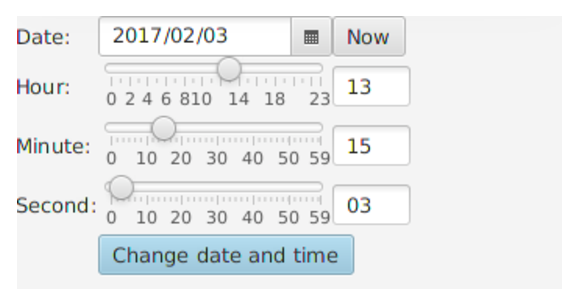
\includegraphics[scale=0.75]{setclock.eps}
	\caption{Setting the clock of the system}
\end{figure}

\begin{figure}[h]
    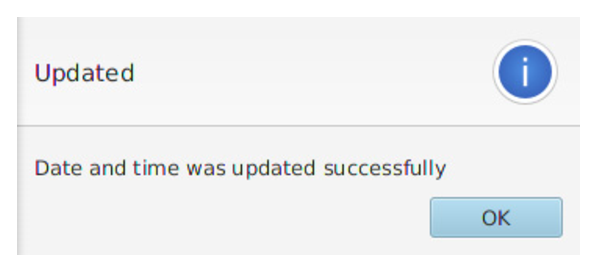
\includegraphics[scale=0.75]{setclock2.eps}
	\caption{Date and time was updated successfuly}
\end{figure}

\section{Login}
\label{operation:Login}

The user enters the system by entering credentials - login and password. The
user has three attemps to enter correct login and password, after three
unsuccessful attempts there is a captcha test. The user has to pass the captcha
test to make a new attempt of authentication.

\begin{description}
	\item \textbf{Parameters:} Login and Password
	\item \textbf{Precondition:} The system is started and the actor is not logged
	in. 
	\item \textbf{Post-condition:} If login and password are correct then the
	actor is logged in the system, otherwise - there is a notification
	of incorrect data and all the administrators are notified of an intrusion
	temptative. After getting incorrect credentials three times in a row the
	system causes a captcha test. 
	\item \textbf{Output messages:} ieMessage: "You are logged in! Welcome
	\ldots"
	
	\item \textbf{Triggering:}
	
	\begin{enumerate}
		\item In the iCrash authentification panel enter login and password, given by
		the supplier/administrator.
		\item Click on the button "Log on"
		\item In case of failure there is a notification of incorrect data.
		\item After three unsuccessful atempts the user has to pass the captcha test
		to try to login one more time.
	\end{enumerate}
\end{description}


\subsection{Login - example}

\begin{figure}[h]
    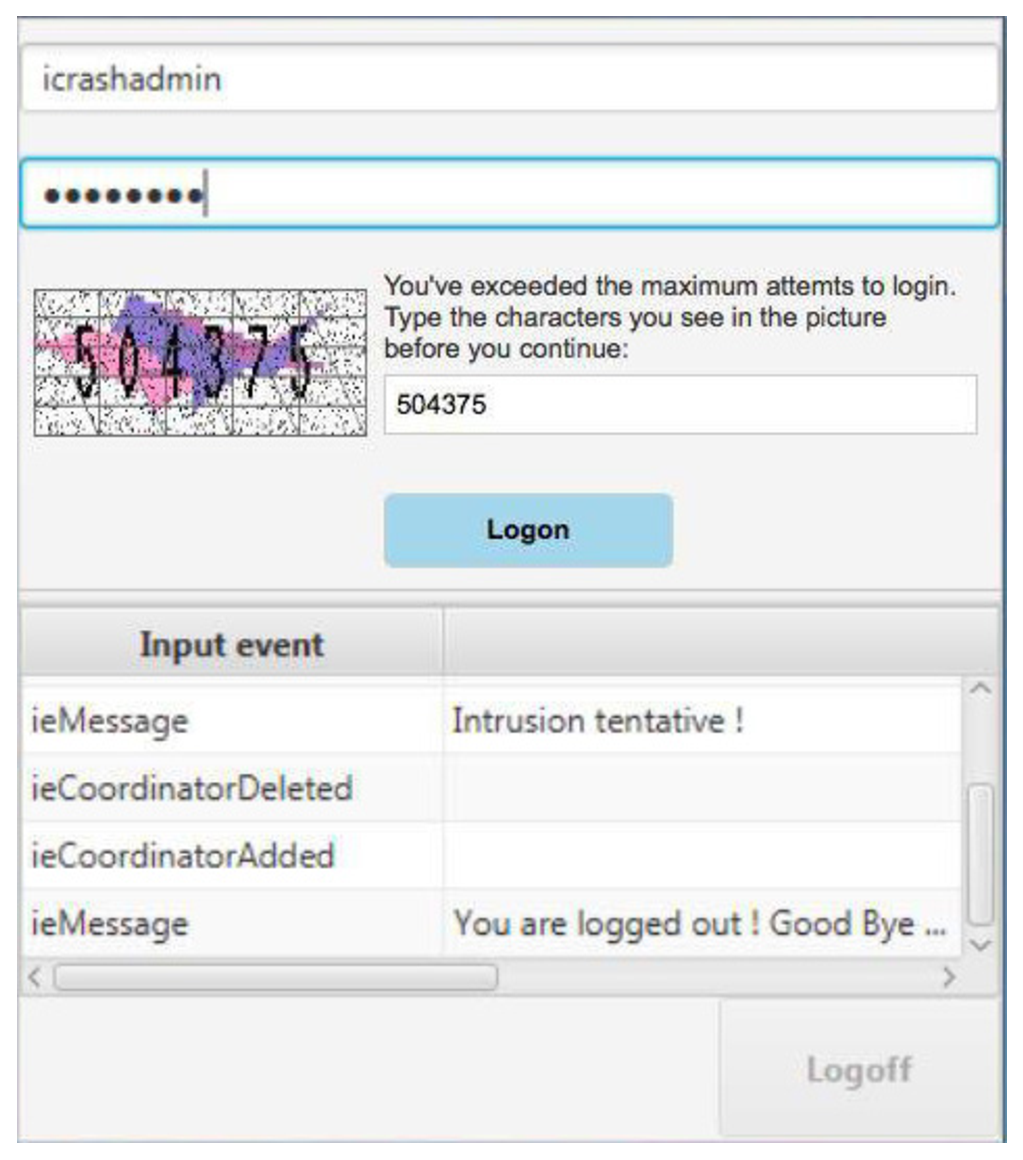
\includegraphics[scale=0.5]{login.eps}
	\caption{Captcha test}
\end{figure}



\section{Logout}
\label{operation:Logout}

The actor loggs out from the system.

\begin{description}
	\item \textbf{Parameters:} None
	\item \textbf{Precondition:} The system is started and the actor is logged in.
	\item \textbf{Post-condition:} The actor is logged out from the system.
	\item \textbf{Output messages:} ieMessage: "You are logged out! Good Bye
	\ldots"
	
	\item \textbf{Triggering:}
	
	\begin{enumerate}
		\item Click on the button "Log off"
	\end{enumerate}
\end{description}



\section{AddCoordinator}
\label{operation:AddCoordinator}

The administrator creates a new coordinator in the system.

\begin{description}
	\item \textbf{Parameters:} CoordinatorID, Login and Password
	\item \textbf{Precondition:} The system is started and the administator is
	logged in. CoordinatorID is a Integer greater than zero and lower or equal to
	5. Length of the Login value is not more than 20 characters. The length of the
	Password is at least 6 characters long.
	\item \textbf{Post-condition:} A new coordinator has been added to the system.
	\item \textbf{Output messages:} "ieCoordinatorAdded"
	
	\item \textbf{Triggering:}
	
	\begin{enumerate}
		\item Click on the button "Add a coordinator' and fill out the entries related
		to the personal information of a coordinator: CoordinatorID, Login and Password.
		\item Click on the button "Create".
	\end{enumerate}
\end{description}

\subsection{AddCoordinator - example}

\begin{figure}
    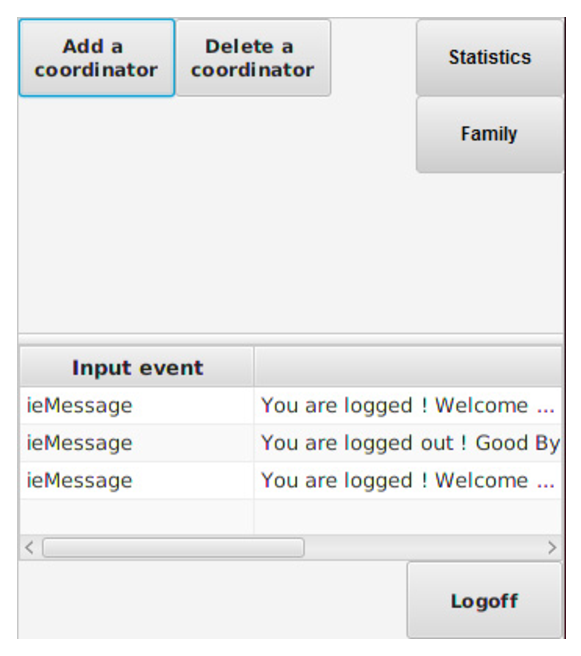
\includegraphics[scale=0.75]{admin.eps}
	\caption{Admins' panel}
\end{figure}

\begin{figure}
    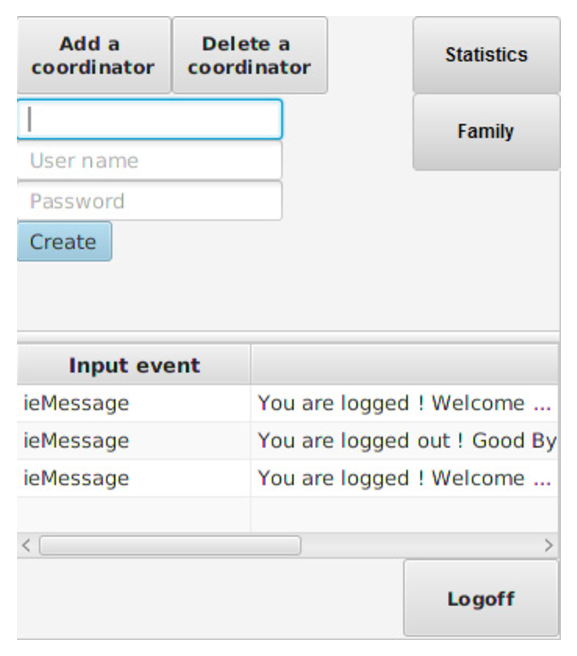
\includegraphics[scale=0.75]{addcoord.eps}
	\caption{Adding a coordinator}
\end{figure}



\section{DeleteCoordinator}
\label{operation:DeleteCoordinator}

The administrator deletes a coordinator from the system.

\begin{description}
	\item \textbf{Parameters:} CoordinatorID
	\item \textbf{Precondition:} The administator is logged in.
	\item \textbf{Post-condition:} The coordinator has been deleted from the
	system.
	\item \textbf{Output messages:} "ieCoordinatorDeleted"
	
	\item \textbf{Triggering:}
	
	\begin{enumerate}
		\item Click on the button "Delete a coordinator' and fill in the ID of the
		coordinator whom to delete.
		\item Click on the button "Delete". %%%% TODO: check the button whether it
		% is "Delete"
	\end{enumerate}
\end{description}


\section{HandleAlert}
\label{operation:HandleAlert}

An coordinator handles alerts received by changing their status.

\begin{description}
	\item \textbf{Parameters:} AlertID 
	\item \textbf{Precondition:} The system is started and the coordinator is
	logged in. 
	\item \textbf{Post-condition:} The status of the alert has been changed.
	\item \textbf{Output messages:} ieMessage: "The Alert is now declared as valid
	(or invalid)!"
	
	\item \textbf{Triggering:}
	
	\begin{enumerate}
		\item Choose an alert from the list and change its status by clicking on the
		button "Validate" or "Invalidate"
	\end{enumerate}
\end{description}

\subsection{HandleAlert - example}

\begin{figure}
    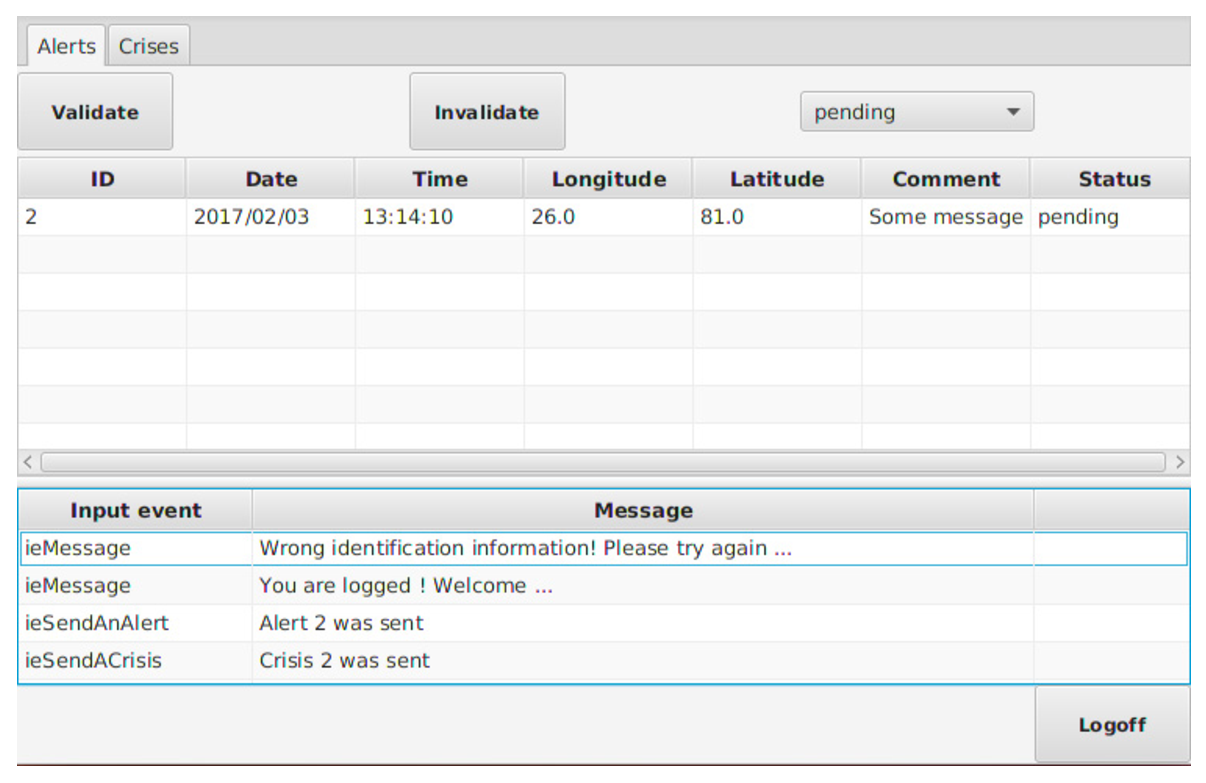
\includegraphics[scale=0.75]{handle_alert.eps}
	\caption{Coordinator panel - alerts}
\end{figure}




\section{GetAlertSet}
\label{operation:GetAlertSet}

An coordinator gets a set of alerts with particular status.

\begin{description}
	\item \textbf{Parameters:} AlertStatus 
	\item \textbf{Precondition:} The system is started and the coordinator is
	logged in.
	\item \textbf{Post-condition:} The list of alerts contains only alerts with chosen status.
	\item \textbf{Output messages:} None
		
	\item \textbf{Triggering:}
	
	\begin{enumerate}
		\item Choose a particular status from the drop-down list.
	\end{enumerate}
\end{description}



\section{GetCrisisSet}
\label{operation:GetCrisisSet}

An coordinator gets a set of crises with particular status.

\begin{description}
	\item \textbf{Parameters:} AlertStatus  
	\item \textbf{Precondition:} The system is started and the coordinator is
	logged in.
	\item \textbf{Post-condition:} The list of crises contains only crises with
	chosen status.
	\item \textbf{Output messages:} None
	
	\item \textbf{Triggering:}
	
	\begin{enumerate}
		\item Choose a particular crisis' status from the drop-down list.
	\end{enumerate}
\end{description}



\section{Alert}
\label{operation:Alert}

An operator of communication company sends an alert received from a human.

\begin{description}
	\item \textbf{Parameters:} HumanKind, Data, Time, PhoneNumber, GPSLocation,
	Comment
	\item \textbf{Precondition:} The system is initialized. Time of the alert is
	earlier than the current time of the system. The value of the latitude part
	of the GPSLocation is a real in the interval [-90.0 , +90.0]. The value of the longitude part
	of the GPSLocation is a	real in the interval [-180.0 , +180.0]. The length of
	the PhoneNumber is from 4 to 30 characters. The length of the Comment is
	not more than 160 characters.
	\item \textbf{Post-condition:} There is an alert with the status - "pending" in
	the list of alerts in coordinator panel. If there were no alerts before with the
	near location to the received alert there is a crisis with
	the same ID as the received alert has, the type - small, the status - pending.
	Else the received alert will be related to the nearest crisis initialized. 
	\item \textbf{Output messages:} None
	
	\item \textbf{Triggering:}
	
	\begin{enumerate}
		\item Choose a type of a person.
		\item Choose a date.
		\item Fill out the entries with the phonenumber, the latitude, the longitude
		and the comment.
		\item Set the time of the alert using scrollbars.
		\item Press on the button "Send alert" or in case of cancel - "Reset form".
	\end{enumerate}
\end{description}

\subsection{Alert - example}

\begin{figure}
    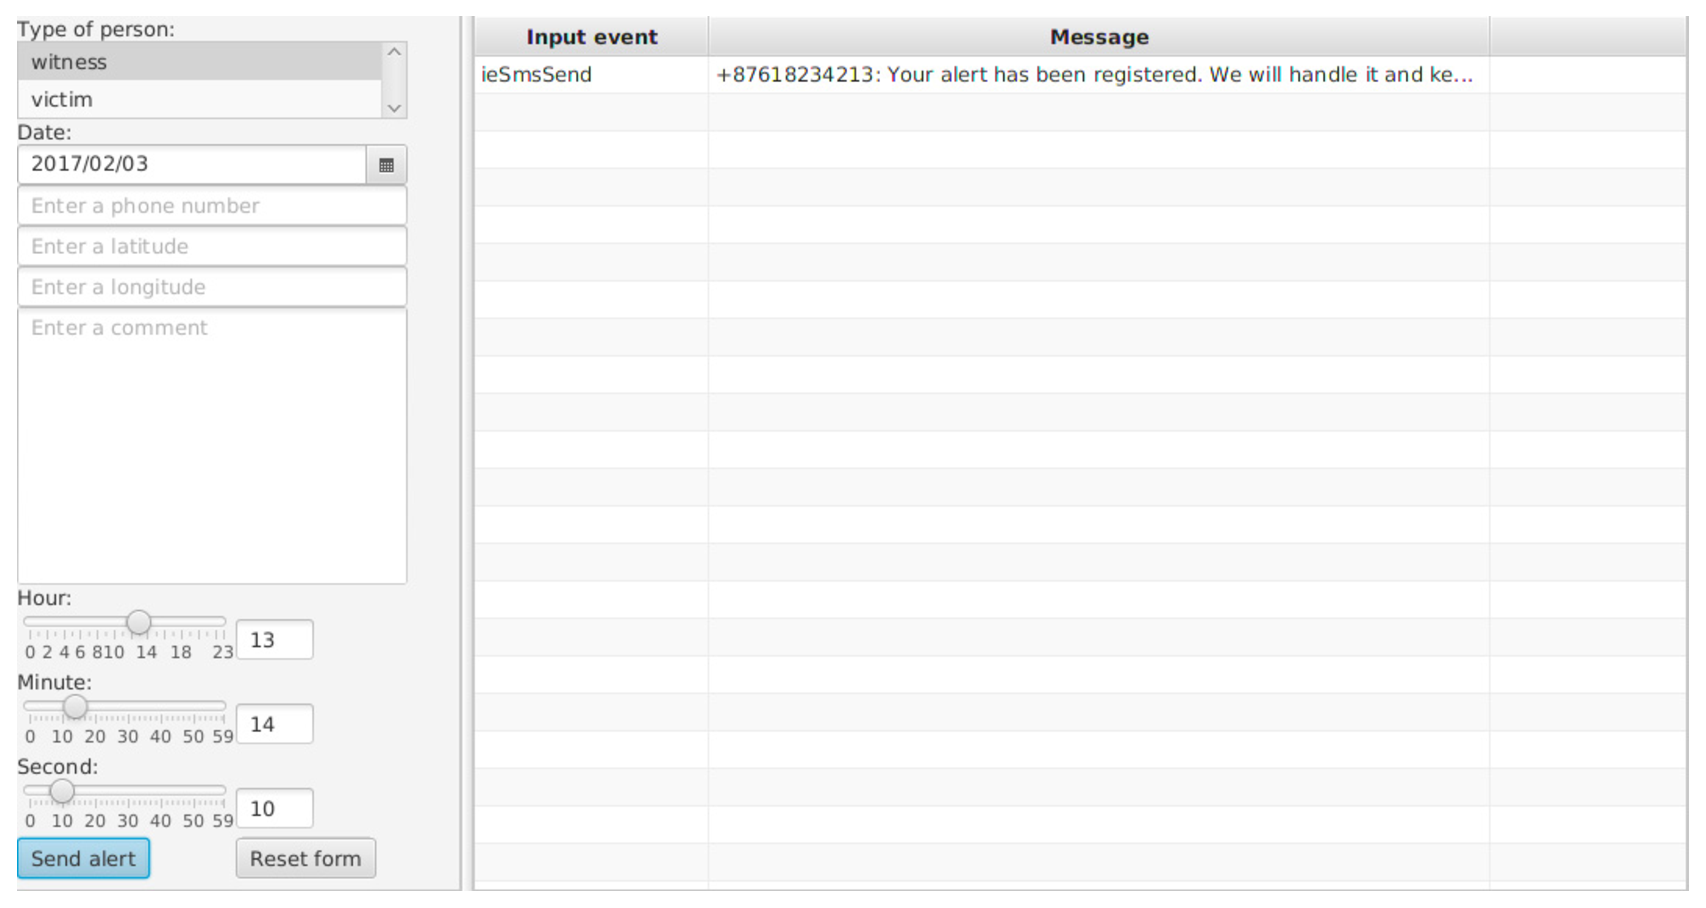
\includegraphics[scale=0.6]{com_company.eps}
	\caption{Communication company panel}
\end{figure}


\section{HandleCrisis}
\label{operation:HandleCrisis}

An coordinator handles a crisis by declaring himself as a handler of the crisis.

\begin{description}
	\item \textbf{Parameters:} CrisisID 
	\item \textbf{Precondition:} The system is started and the coordinator is
	logged in.
	\item \textbf{Post-condition:} The status of the alert has been changed to
	"handled". The crisis is associated to the coordinator who has handled the crisis.
	All the related alerts are sent to the coordinator. If the crisis was already
	handled its handler is updated to the new one and the previous handler is
	notified. A message to the related human is sent through the communication
	company.
	\item \textbf{Output messages:} ieMessage: "You are now considered as handling
	the crisis".
	
	\item \textbf{Triggering:}
	
	\begin{enumerate}
		\item Choose an alert from the list and press on the button "Handle crisis".
	\end{enumerate}
\end{description}

\subsection{HandleCrisis - example}

\begin{figure}
    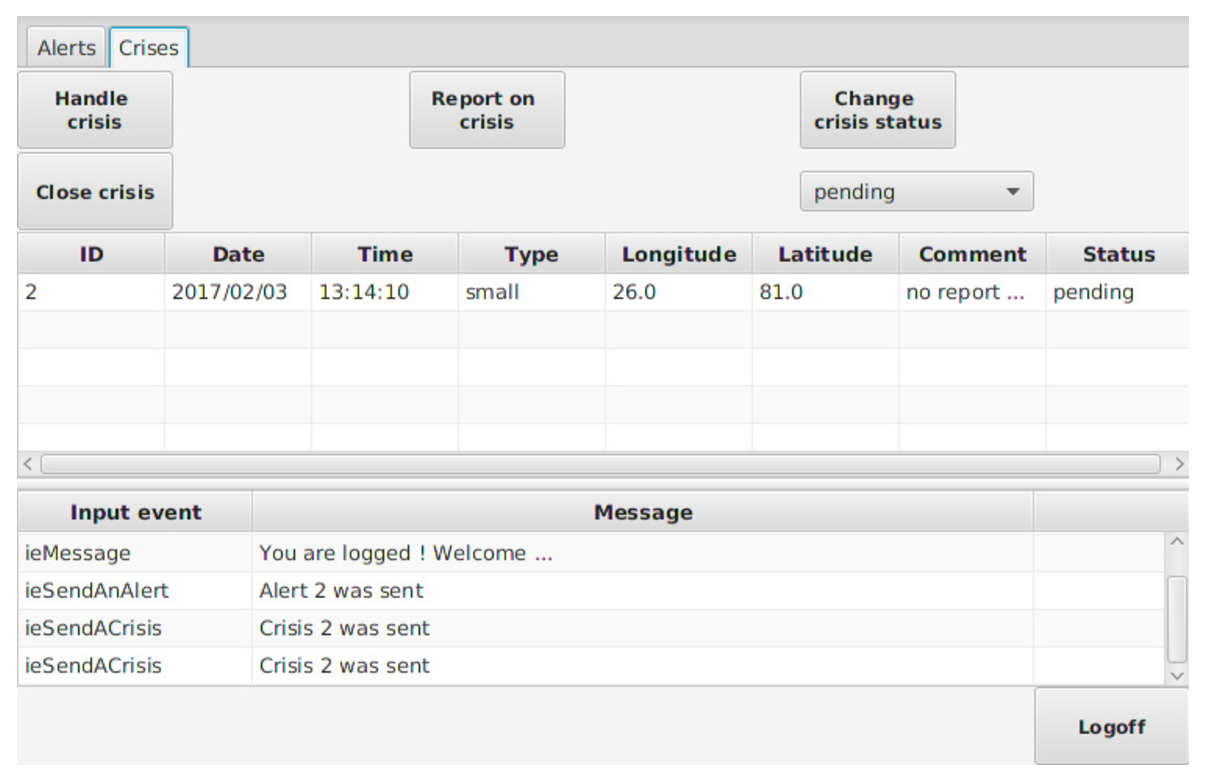
\includegraphics[scale=0.6]{crisis.eps}
	\caption{Coordinator panel - crises}
\end{figure}

\section{ReportOnCrisis}
\label{operation:ReportOnCrisis}

An coordinator updates the textual information for a crisis.

\begin{description}
	\item \textbf{Parameters:} CrisisID and Comment
	\item \textbf{Precondition:} The system is started and the coordinator is
	logged in. The length of the comment value is not more than 160 characters.
	\item \textbf{Post-condition:} The comment attribute of the crisis has been
	updated.
	\item \textbf{Output messages:} ieMessage: "The crisis comment has
	been updated "'
	
	\item \textbf{Triggering:}
	
	\begin{enumerate}
		\item Choose an alert from the list and press on the button "Report on crisis".
		\item Enter in the text field a report and press on the button "Report" or in case of cancel - "Cancel"
	\end{enumerate}
\end{description}


\section{SetStatusCrisis}
\label{operation:SetStatusCrisis}

An coordinator sets the status of a crisis.

\begin{description}
	\item \textbf{Parameters:} CrisisID and CrisisStatus
	\item \textbf{Precondition:} The system is started and the coordinator is
	logged in.
	\item \textbf{Post-condition:} The status of the alert has been changed.
	\item \textbf{Output messages:} ieMessage: "The crisis status has been updated !".
	
	\item \textbf{Triggering:}
	
	\begin{enumerate}
		\item Choose an alert from the list and press on the button "Change crisis
		status".
		\item Choose the status from the drop-box and press on the button "Change
		crisis" or in case of cancel - "Cancel"
	\end{enumerate}
\end{description}


\section{CloseCrisis}
\label{operation:CloseCrisis}

An coordinator closes a crisis.

\begin{description}
	\item \textbf{Parameters:} CrisisID
	\item \textbf{Precondition:} The system is started and the coordinator is
	logged in.
	\item \textbf{Post-condition:} The status of the alert has been changed to
	"closed". There is no handler associated to the closed crisis.
	\item \textbf{Output messages:} ieMessage: "The crisis is now closed !".
	
	\item \textbf{Triggering:}
	
	\begin{enumerate}
		\item Choose an alert from the list and press on the button "Close crisis".
	\end{enumerate}
\end{description}

\section{GetTimeStatistics}
\label{operation:GetTimeStatistics}

The administrator gets the list of alerts and crises on the concrete date or
within a defined period with extra time statistics.
When the alert was validated/invalidated; when the crisis was handled; all the times when the status was changed; when reported; when closed.
Also the administrator gets an average time for validating alerts and closing crises.


\begin{description}
	\item \textbf{Parameters:} Date/Period
	\item \textbf{Precondition:} The system is started and the administrator is
	logged in.
	\item \textbf{Post-condition:} There is the list of alerts/crises with all the
	time statistics and the average time for processing.
	\item \textbf{Output messages:} None
	
	\item \textbf{Triggering:}
	
	\begin{enumerate}
		\item In the admin panel press on the button "Statistics".
		\item Press on the button "Alerts" or "Crises".
		\item Choose the date or press on the radio button "Period of time" for
		chossing a period.
		\item To get statistics - prress on the button "Get statistics".
		\item To close the statistics panel - press on the button "Close".
	\end{enumerate}
\end{description}

\subsection{GetTimeStatistics - example}

\begin{figure}[h]
    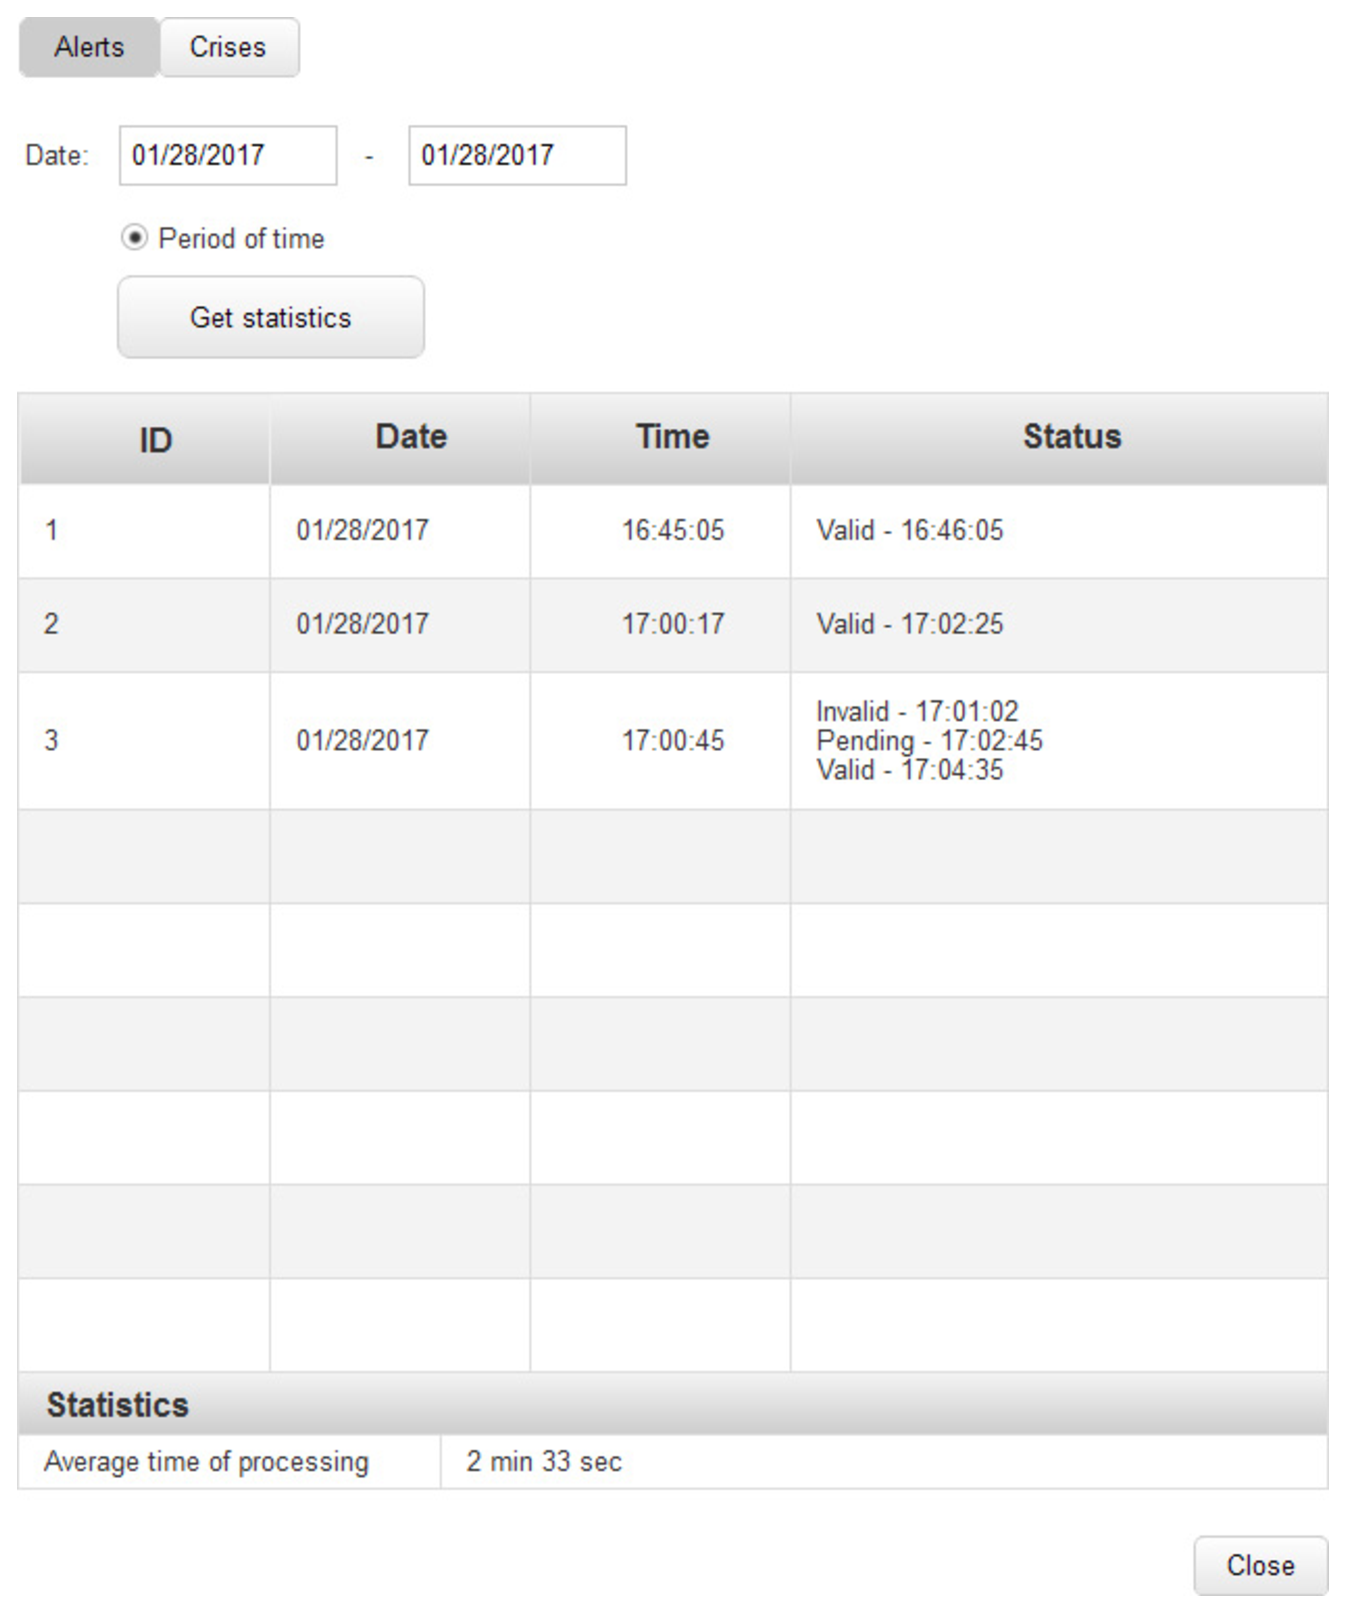
\includegraphics[scale=0.5]{alert_stats.eps}
	\caption{Time statistics of alerts}
\end{figure}

\begin{figure}[h] 
    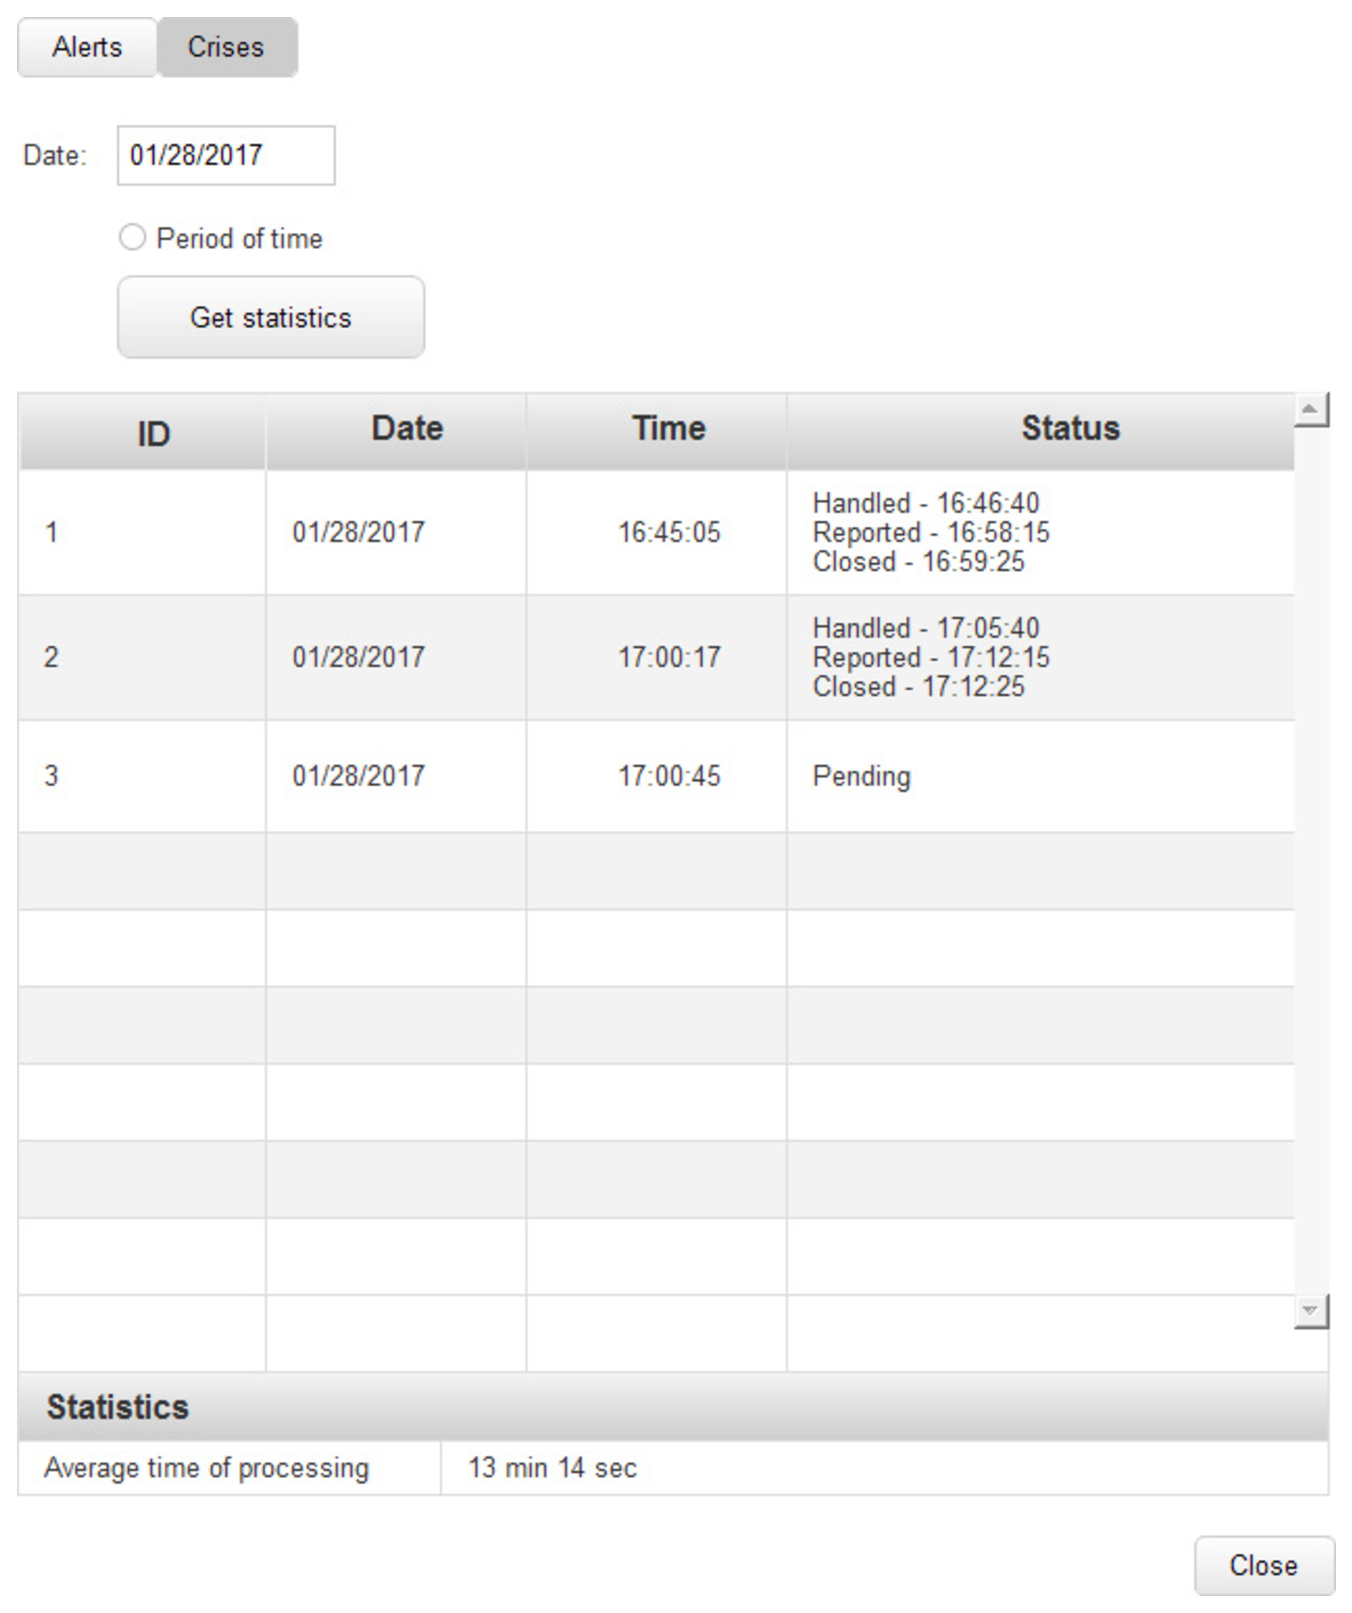
\includegraphics[scale=0.5]{crisis_stats.eps}
	\caption{Time statistics of crises}
\end{figure}



